\documentclass[tikz, border=3mm]{standalone}
\usepackage{tikz}
\usetikzlibrary{positioning,fit,arrows.meta,backgrounds}

\tikzset{
  module/.style={
    draw, rounded corners,
    minimum width=2cm,
    minimum height=7mm,
    font=\sffamily
  },
  container/.style={
    draw, rounded corners,
    minimum width=2cm,
    minimum height=5cm,
    font=\sffamily
  },
  small/.style={
    draw, rounded corners,
    minimum height=2.5cm,
    font=\sffamily
  },
  >=LaTeX
}

\begin{document}
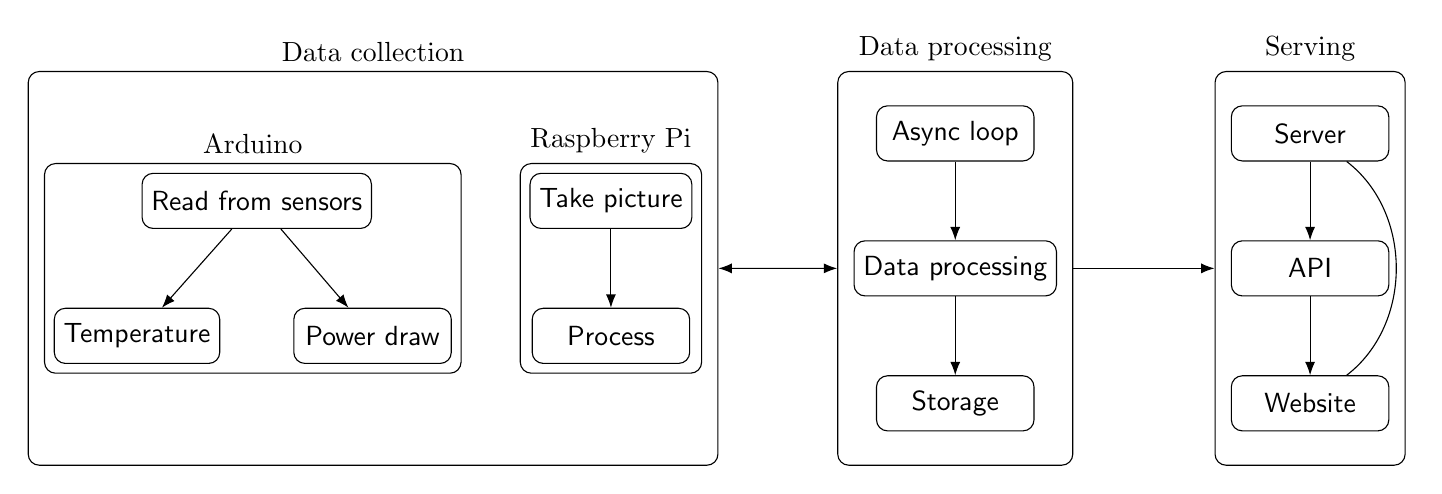
\begin{tikzpicture}[auto]
  % Arduino box
  \node[module] (Read) {Read from sensors};
  \node[module, below left=1cm and -1cm of Read] (Temp) {Temperature};
  \node[module, below right=1cm and -1cm of Read] (Power) {Power draw};
  \node[small,fit=(Read) (Temp) (Power), draw, label={Arduino}] (SensorBox) {};
  \draw[->] (Read)--(Temp);
  \draw[->] (Read)--(Power);
  % Raspberry Pi processing box
  \node[module, right=2cm of Read] (Camera) {Take picture};
  \node[module, below=of Camera] (CamProcess) {Process};
  \node[small, fit=(Camera) (CamProcess), draw, label={Raspberry Pi}] (Pi2Box) {};
  \draw[->] (Camera)--(CamProcess);

  % Data collection box
  \node[container, fit=(SensorBox) (Pi2Box),
  draw, inner xsep=2mm, inner ysep=.5cm,
  label={Data collection}] (DataCollectionBox) {};

  % Data processing box
  \node[module, above right=-1.15cm and 2cm of DataCollectionBox] (AsyncLoop) {Async loop};
  \node[module, below=of AsyncLoop] (Data) {Data processing};
  \node[module, below=of Data] (Storage) {Storage};
  \node[container, fit={(AsyncLoop) (Data) (Storage)},
        draw, inner sep=2mm,
        label={Data processing}]
        (MainBox) {};
  \draw[->] (AsyncLoop)--(Data);
  \draw[->] (Data)--(Storage);

  % Connect main loop and async loop
  \draw[<->] (DataCollectionBox)--(MainBox);

  % Serve box
  \node[module, right=2cm of {AsyncLoop-|MainBox.east}] (Server) {Server};
  \node[module, below=of Server] (API) {API};
  \node[module, below=of API] (Website) {Website};
  \node[container, fit={(Server) (API) (Website)}, draw, inner sep=2mm, label={Serving}] (ServeBox) {};
  \draw[->] (Server)--(API);
  \draw[] (Server) edge[bend left=52.5] node [left] {} (Website);
  \draw[->] (API)--(Website);
  \draw[->] (MainBox)--(ServeBox);
\end{tikzpicture}
\end{document}
%%% Local Variables:
%%% mode: latex
%%% TeX-master: t
%%% End:
